%\documentclass[12pt]{article}

\questionheader{ex:s3.6}


%%%%%%%%%%%%%%%%%%
\subsection*{\Conceptual}
%%%%%%%%%%%%%%%%%%

%%%%%%%%%%%%%%%%%%%%%%%%%%%%%%%%%%%%%%%%%
\begin{question}
Use $(r,\theta,z)$ to denote cylindrical coordinates.
\begin{enumerate}[(a)]
\item
Draw $r=0$.
\item
Draw $r=1$.
\item 
Draw $\theta=0$.
\item
Draw $\theta=\nicefrac{\pi}{4}$.
\end{enumerate}

\end{question}

%\begin{hint}
%
%\end{hint}

\begin{answer}
(a), (b)
\begin{center}
   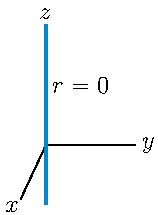
\includegraphics{cylR0.pdf}\qquad\qquad
   \raisebox{-0.05\height}{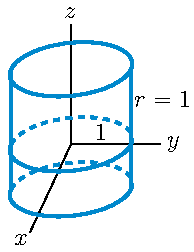
\includegraphics[scale=1.0]{cylR.pdf}}
\end{center}

(c), (d)
\begin{center}
   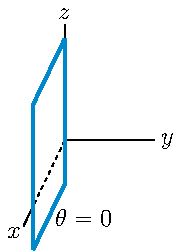
\includegraphics{cylTh0.pdf}\qquad\qquad
   \raisebox{0.0\height}{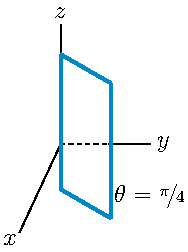
\includegraphics[scale=1.0]{cylTh.pdf}}
\end{center}

\end{answer}

\begin{solution}
(a), (b) Since the cylindrical coordinate $r(x,y,z)$ of a point $(x,y,z)$ is
the distance, $\sqrt{x^2+y^2}$, from $(x,y,z)$ to the $z$-axis, the sets
\begin{align*}
\Set{(x,y,z)}{r(x,y,z)=0}
&=\Set{(x,y,z)}{x^2+y^2=0}
=\Set{(x,y,z)}{x=y=0} \\
&=\text{the $z$-axis} \\
\Set{(x,y,z)}{r(x,y,z)=1}
&=\Set{(x,y,z)}{x^2+y^2=1} \\
&=\text{the cylinder of radius $1$ centred on the $z$-axis}
\end{align*} 
\begin{center}
   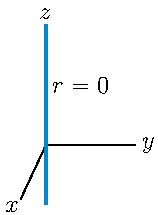
\includegraphics{cylR0.pdf}\qquad\qquad
   \raisebox{-0.05\height}{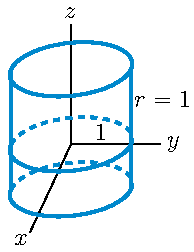
\includegraphics[scale=1.0]{cylR.pdf}}
\end{center}

(c), (d)
Since the cylindrical coordinate $\theta(x,y,z)$ of a point $(x,y,z)$ is
the angle between the positive $x$-axis and the line from $(0,0,0)$ 
to $(x,y,0)$, the sets
\begin{align*}
\Set{(x,y,z)}{\theta(x,y,z)=0}
&=\text{the half of the $xz$-plane with $x>0$} \\
\Set{(x,y,z)}{\theta(x,y,z)=\nicefrac{\pi}{4}}
&=\text{the half of the plane $y=x$ with $x>0$}
\end{align*} 
\begin{center}
   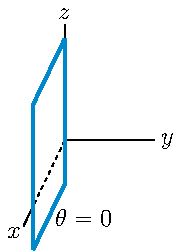
\includegraphics{cylTh0.pdf}\qquad\qquad
   \raisebox{0.0\height}{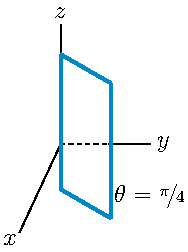
\includegraphics[scale=1.0]{cylTh.pdf}}
\end{center}
\end{solution}


%%%%%%%%%%%%%%%%%%%%%%%%%%%%%%%%%%%%%%%%%
\begin{question}
Sketch the points with the specified cylindrical coordinates.
\begin{enumerate}[(a)]
\item
$r=1$, $\theta=0$, $z=0$
\item
$r=1$, $\theta=\frac{\pi}{4}$, $z=0$
\item
$r=1$, $\theta=\frac{\pi}{2}$, $z=0$
\item
$r=0$, $\theta=\pi$, $z=1$
\item
$r=1$, $\theta=\frac{\pi}{4}$, $z=1$
\end{enumerate}

\end{question}

%\begin{hint}
%
%\end{hint}

\begin{answer}
\begin{center}
   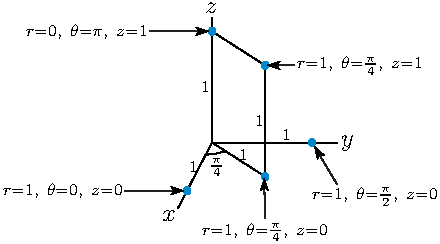
\includegraphics{cylP1.pdf}
\end{center}
\end{answer}

\begin{solution}
The sketch is below. To help build up this sketch, it is useful to 
recall the following facts.
\begin{itemize}
\item
The cylindrical coordinate $r$ is the distance of the point from the $z$-axis.
In particular all points with $r=0$ lie on the $z$-axis (for all values of $\theta$).
\item
The cylindrical coordinate $z$ is the distance of the point from the $xy$-plane.
In particular all points with $z=0$ lie on the $xy$-plane.
\end{itemize}
\begin{center}
   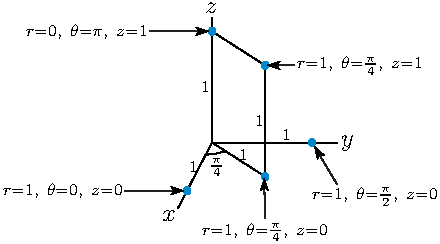
\includegraphics{cylP1.pdf}
\end{center}
\end{solution}

%%%%%%%%%%%%%%%%%%%%%%%%%%%%%%%%%%%%%%%%%
\begin{question}
Convert from cylindrical to Cartesian coordinates.
\begin{enumerate}[(a)]
\item
$r=1$, $\theta=0$, $z=0$
\item
$r=1$, $\theta=\frac{\pi}{4}$, $z=0$
\item
$r=1$, $\theta=\frac{\pi}{2}$, $z=0$
\item
$r=0$, $\theta=\pi$, $z=1$
\item
$r=1$, $\theta=\frac{\pi}{4}$, $z=1$
\end{enumerate}

\end{question}

%\begin{hint}
%
%\end{hint}

\begin{answer}
(a) $(1,0,0)$\qquad
(b) $\left(\frac{1}{\sqrt{2}},\frac{1}{\sqrt{2}},0\right)$\qquad
(c) $(0,1,0)$\qquad
(d) $(0,0,1)$\qquad
(e) $\left(\frac{1}{\sqrt{2}},\frac{1}{\sqrt{2}},1\right)$
\end{answer}

\begin{solution}
(a) When $\theta=0$,  $\sin\theta=0$ and $\cos\theta=1$, so that
the polar coordinates $r=1$, $\theta=0$, $z=0$ correspond to the Cartesian
coordinates
\begin{equation*}
(x,y,z) = (r\cos\theta,r\sin\theta,z)
        = (1\times\cos 0,\  1\times\sin 0,\ 0)
        =(1,0,0)
\end{equation*}

(b) When $\theta=\frac{\pi}{4}$,  $\sin\theta=\cos\theta=\frac{1}{\sqrt{2}}$, 
so that the polar coordinates $r=1$, $\theta=\frac{\pi}{4}$, $z=0$ correspond 
to the Cartesian coordinates
\begin{equation*}
(x,y,z) = (r\cos\theta,r\sin\theta,z)
  = \left(1\times\cos \frac{\pi}{4},\  1\times\sin \frac{\pi}{4},\ 0\right)
  = \left(\frac{1}{\sqrt{2}},\frac{1}{\sqrt{2}},0\right)
\end{equation*}

(c) When $\theta=\frac{\pi}{2}$,  $\sin\theta=1$ and $\cos\theta=0$, 
so that the polar coordinates $r=1$, $\theta=\frac{\pi}{2}$, $z=0$ correspond 
to the Cartesian coordinates
\begin{equation*}
(x,y,z) = (r\cos\theta,r\sin\theta,z)
  = \left(1\times\cos \frac{\pi}{2},\  1\times\sin \frac{\pi}{2},\ 0\right)
  = (0,1,0)
\end{equation*}

(d) When $\theta=\pi$,  $\sin\theta=0$ and $\cos\theta=-1$, 
so that the polar coordinates $r=0$, $\theta=\pi$, $z=1$ correspond 
to the Cartesian coordinates
\begin{equation*}
(x,y,z) = (r\cos\theta,r\sin\theta,z)
  = \left(0\times\cos\pi,\  0\times\sin\pi,\ 1\right)
  = (0,0,1)
\end{equation*}

(e) When $\theta=\frac{\pi}{4}$,  $\sin\theta=\cos\theta=\frac{1}{\sqrt{2}}$, 
so that the polar coordinates $r=1$, $\theta=\frac{\pi}{4}$, $z=1$ correspond 
to the Cartesian coordinates
\begin{equation*}
(x,y,z) = (r\cos\theta,r\sin\theta,z)
  = \left(1\times\cos \frac{\pi}{4},\  1\times\sin \frac{\pi}{4},\ 1\right)
  = \left(\frac{1}{\sqrt{2}},\frac{1}{\sqrt{2}},1\right)
\end{equation*}

\end{solution}

%%%%%%%%%%%%%%%%%%%%%%%%%%%%%%%%%%%%%%%%%
\begin{question}
Convert from Cartesian to cylindrical coordinates.
\begin{enumerate}[(a)]
\item $(1,1,2)$
\item $(-1,-1,2)$
\item $(-1,\sqrt{3}, 0)$
\item $(0,0,1)$
\end{enumerate}

\end{question}

%\begin{hint}
%
%\end{hint}

\begin{answer}
(a) $r=\sqrt{2}$, $z=2$, $\theta=\frac{\pi}{4}$ (plus possibly
any integer multiple of $2\pi$)

(b) $r=\sqrt{2}$, $z=2$, $\theta=\frac{5\pi}{4}$ (plus possibly
any integer multiple of $2\pi$)

(c) $r=2$, $z=0$, $\theta=\frac{2\pi}{3}$ (plus possibly
any integer multiple of $2\pi$)

(d) $r=0$, $z=1$, $\theta=\text{arbitrary}$

\end{answer}

\begin{solution}
(a) The cylindrical coordinates must obey
\begin{equation*}
1=x=r\cos\theta\qquad
1=y=r\sin\theta\qquad
2=z
\end{equation*}
So $z=2$, $r=\sqrt{1^2+1^2}=\sqrt{2}$ and $\tan\theta=\frac{y}{x}
=\frac{1}{1}=1$. Recall that $\tan\left(\frac{\pi}{4}+k\pi\right)=1$
for all integers $k$.  As $(x,y)=(1,1)$ lies in the first quadrant,
$0\le\theta\le\frac{\pi}{2}$. So $\theta=\frac{\pi}{4}$ (plus possibly
any integer multiple of $2\pi$). 

(b) The cylindrical coordinates must obey
\begin{equation*}
-1=x=r\cos\theta\qquad
-1=y=r\sin\theta\qquad
2=z
\end{equation*}
So $z=2$, $r=\sqrt{(-1)^2+(-1)^2}=\sqrt{2}$ and $\tan\theta=\frac{y}{x}
=\frac{-1}{-1}=1$. Recall that $\tan\left(\frac{\pi}{4}+k\pi\right)=1$
for all integers $k$. As $(x,y)=(-1,-1)$ lies in the third quadrant,
$\pi\le\theta\le\frac{3\pi}{2}$. So $\theta=\frac{5\pi}{4}$ (plus possibly
any integer multiple of $2\pi$).

(c) The cylindrical coordinates must obey
\begin{equation*}
-1=x=r\cos\theta\qquad
\sqrt{3}=y=r\sin\theta\qquad
0=z
\end{equation*}
So $z=0$, $r=\sqrt{(-1)^2+\big(\sqrt{3}\big)^2}=2$ and 
$\tan\theta=\frac{y}{x} =\frac{\sqrt{3}}{-1}=-\sqrt{3}$. 
Recall that $\tan\left(\frac{2\pi}{3}+k\pi\right)=-\sqrt{3}$
for all integers $k$.
As $(x,y)=(-1,\sqrt{3})$ lies in the second quadrant,
$\frac{\pi}{2}\le\theta\le\pi$. So $\theta=\frac{2\pi}{3}$ (plus possibly
any integer multiple of $2\pi$). 

(d) The cylindrical coordinates must obey
\begin{equation*}
0=x=r\cos\theta\qquad
0=y=r\sin\theta\qquad
1=z
\end{equation*}
So $z=0$, $r=\sqrt{0^2+0^2}=0$ and 
$\theta$ is completely arbitrary. 

\end{solution}


%%%%%%%%%%%%%%%%%%%%%%%%%%%%%%%%%%%%%%%%%
\begin{question}
Rewrite the following equations in cylindrical coordinates.
\begin{enumerate}[(a)]
\item $z=2xy$
\item $x^2+y^2+z^2=1$
\item $(x-1)^2 + y^2 =1$
\end{enumerate}

\end{question}

%\begin{hint}
%
%\end{hint}

\begin{answer}
(a) $z=r^2\sin(2\theta)$\qquad
(b) $r^2+z^2=1$\qquad
(c) $r=2\cos\theta$

\end{answer}

\begin{solution}
(a) As $x=r\cos\theta$ and $y=r\sin\theta$,
\begin{equation*}
z=2xy
\iff z=2r^2\cos\theta\sin\theta = r^2\sin(2\theta)
\end{equation*}

(b) As $x=r\cos\theta$ and $y=r\sin\theta$,
\begin{equation*}
x^2+y^2+z^2=1
\iff r^2\cos^2\theta+r^2\sin^2\theta + z^2 =1 
\iff r^2+z^2=1
\end{equation*}

(c) As $x=r\cos\theta$ and $y=r\sin\theta$,
\begin{align*}
(x-1)^2 + y^2 =1
&\iff (r\cos\theta-1)^2 + (r\sin\theta)^2 =1 \\
&\iff r^2\cos^2\theta -2r\cos\theta +1 + r^2\sin^2\theta = 1 \\
&\iff r^2=2r\cos\theta
\iff r=2\cos\theta\text{ or }r=0 \\
&\iff r=2\cos\theta
\end{align*}
Note that the solution $r=0$ is included in $r=2\cos\theta$ --- just choose $\theta=\frac{\pi}{2}$.

\end{solution}

%%%%%%%%%%%%%%%%%%%%%%%%%%%%
%\Instructions{Questions~\ref{prob_s1.0first} through \ref{prob_s1.0last} provide practice with.}
%%%%%%%%%%%%%%%%%%%%

%%%%%%%%%%%%%%%%%%
\subsection*{\Procedural}
%%%%%%%%%%%%%%%%%%

%%%%%%%%%%%%%%%%%%%%%%%%%%%%%%%%
\begin{question}
Use cylindrical coordinates to evaluate the volumes of each of the following
regions.
\begin{enumerate}[(a)]
\item
Above the $xy$--plane, inside the cone $z=2a-\sqrt{x^2+y^2}$ and
inside the cylinder $x^2+y^2=2ay$.
\item
Above the $xy$--plane, under the paraboloid $z=1-x^2-y^2$ and
in the wedge $-x\le y\le \sqrt{3}x$.
\item
Above the paraboloid $\ z=x^2+y^2\ $ and below the plane $\ z=2y$.
\end{enumerate}
\end{question}

%\begin{hint}
%
%\end{hint}

\begin{answer}
(a) $a^3\big(2\pi-\frac{32}{9}\big)$ \qquad
(b) $\frac{7}{48}\pi$\qquad
(c) $\frac{\pi}{2}$
\end{answer}

\begin{solution}
 (a) In cylindrical coordinates, the cone $z=2a-\sqrt{x^2+y^2}$ is $z=2a-r$
and the cylinder $x^2+y^2=2ay$ is $r^2=2ar\sin\theta$ or $r=2a\sin\theta$.
The figures below show the parts of the cone, the cylinder and
the intersection, respectively, that are in the first octant. 
\begin{center}
     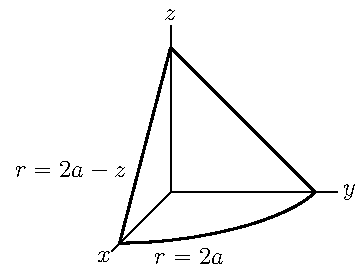
\includegraphics[scale=0.9]{domainCylinderConea.pdf}
     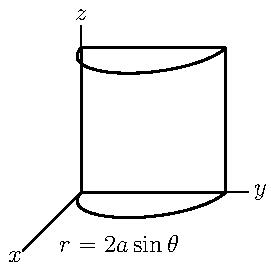
\includegraphics[scale=0.9]{domainCylinderConeb.pdf}
     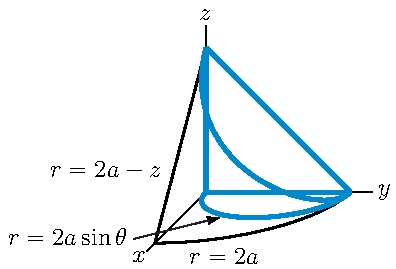
\includegraphics[scale=0.9]{domainCylinderCone.pdf}
\end{center}
The specified region is
\begin{equation*}
V=\Set{(r\cos\theta\,,\,r\sin\theta\,,\,z)}
           {0\le\theta\le\pi,\ r\le 2a\sin\theta,\ 0\le z\le 2a-r}
\end{equation*}
By symmetry under $x\rightarrow -x$, the full volume is twice the
volume in the first octant. 

So the
\begin{align*}
\text{Volume} 
&= 2\int_0^{{\pi\over 2}} \dee{\theta}\int_0^{2a\sin\theta}\dee{r}\ r
           \int_0^{2a -r}\dee{z} \displaybreak[0]\\
&= 2\int_0^{{\pi\over 2}} \dee{\theta}\int_0^{2a\sin\theta}\dee{r}\ r(2a-r) 
              \displaybreak[0]\\
&= 2\int_0^{{\pi\over 2}} \dee{\theta}\ 
             \left[4a^3\sin^2\theta-\frac{8a^3}{3}\sin^3\theta\right] 
               \displaybreak[0]\\
&= 8a^3\left[\int_0^{{\pi\over 2}} \dee{\theta}\ \frac{1-\cos(2\theta)}{2}
             +\frac{2}{3}\int^0_1 \dee{t}\ \big(1-t^2\big)\right]
\qquad\text{where $t=\cos\theta$} \\
&= 8a^3\left[\frac{\pi}{4}-\frac{2}{3}\left(1-\frac{1}{3}\right)\right]
=a^3\big(2\pi-\frac{32}{9}\big)
\end{align*}
For an efficient, sneaky, way to evaluate 
$\int_0^{{\pi\over 2}} \dee{\theta}\ \sin^2\theta$, 
see Remark \eref{CLP200}{rem sneaky} in the CLP-3 text.

(b) The domain of integration is
\begin{equation*}
V = \Set{(x,y,z)}{-x\le y\le \sqrt{3}x,\ 0\le z \le 1-x^2-y^2}
\end{equation*}
Recall that in polar coordinates $\frac{y}{x}=\tan\theta$.
So the boundaries of the wedge $-x\le y\le \sqrt{3}x$, or equivalently
$-1\le\frac{y}{x}\le\sqrt{3}$, correspond, in polar coordinates, 
to $\theta=\tan^{-1}(-1)=-\frac{\pi}{4}$ and $\theta=\tan^{-1}\sqrt{3}=\frac{\pi}{3}$. In cylindrical coordinates,
the paraboloid $z=1-x^2-y^2$ becomes $z=1-r^2$. There are $z$'s that obey
$0\le z\le 1-r^2$ if and only if $r\le 1$. So, in cylindrical coordinates,
\begin{equation*}
V = \Set{(r\cos\theta,r\sin\theta,z)}
              {-\tfrac{\pi}{4}\le \theta\le \tfrac{\pi}{3},\ 
                  0\le r\le 1,\ 0\le z \le 1-r^2}
\end{equation*}
and
\begin{align*}
\text{Volume} 
&= \int_{-{\pi\over 4}}^{{\pi\over 3}} \dee{\theta}\int_0^1\dee{r}\ r
             \int_0^{1 -r^2}\dee{z}
= \left(\frac{\pi}{3}+\frac{\pi}{4}\right)\int_0^1\dee{r}\ r(1-r^2)
= \frac{7}{12}\pi\left(\frac{1}{2}-\frac{1}{4}\right)
= \frac{7}{48}\pi
\end{align*}

(c) The region is 
\begin{equation*}
V = \Set{(x,y,z)}{x^2+y^2\le z\le 2y}
\end{equation*}
There are $z$'s that obey $x^2+y^2\le z\le 2y$ if and only if
\begin{align*}
x^2+y^2\le 2y
&\iff x^2+y^2-2y \le 0
 \iff x^2 + (y-1)^2 \le 1
\end{align*}
This disk is sketched in the figure
\begin{center}
     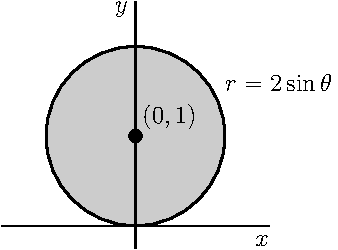
\includegraphics{domain2bis.pdf}
\end{center}
In cylindrical coordinates, 
\begin{itemize}
\item
the bottom, $z=x^2+y^2$, is $z=r^2$, 
\item
the top, $z=2y$, is $z=2r\sin\theta$, and 
\item
the disk $x^2+y^2\le 2y$ is $r^2\le 2r\sin\theta$, or equivalently $r\le2\sin\theta$, 
\end{itemize}
so that, looking at the figure above,
\begin{equation*}
V = \Set{(r\cos\theta,r\sin\theta,z)}{0\le\theta\le\pi,
                \ 0\le r\le 2\sin\theta,\ r^2\le z\le 2r\sin\theta}
\end{equation*}
By symmetry under $x\rightarrow -x$, 
the full volume is twice the volume in the first octant so that
\begin{align*}
\text{Volume} 
&= 2\int_{0}^{{\pi\over 2}} \dee{\theta}\int_0^{2\sin\theta}\dee{r}\ r\int_{r^2}^{2r\sin\theta}\dee{z}
= 2\int_{0}^{{\pi\over 2}} \dee{\theta}\int_0^{2\sin\theta}\dee{r}\ r(2r\sin\theta-r^2)\cr
&= 2\int_{0}^{{\pi\over 2}} \dee{\theta}\ \left(\frac{2^4}{3}-\frac{2^4}{4}\right)\sin^4\theta
%= 2\frac{2^4}{12}\frac{3}{16}\pi
%=\frac{\pi}{2}
\end{align*}
To integrate\footnote{For a general discussion of trigonometric integrals see
\S\eref{CLP101}{sec trigint} in the CLP-2 text. In particular the integral  
$\int \cos^4 x\ \dee{x}$ is evaluated in Example \eref{CLP101}{eg:TRGINTc} 
in the CLP-2 text.} 
$\sin^4\theta$, we use the double angle formulae
$\sin^2 x= \frac{1-\cos(2x)}{2}$ and $\cos^2 x= \frac{1+\cos(2x)}{2}$
to write
\begin{align*}
  \sin^4\theta &= \left[ \frac{1-\cos(2\theta)}{2} \right]^2 \\
   &= \frac{1}{4} - \frac{1}{2} \cos(2\theta) + \frac{1}{4}\cos^2(2\theta)\\
  &= \frac{1}{4} - \frac{1}{2} \cos(2\theta) + \frac{1}{8}\left(1 + \cos(4\theta) \right)\\
  &= \frac{3}{8} - \frac{1}{2} \cos(2\theta) + \frac{1}{8}\cos(4\theta)
\end{align*}
So
\begin{align*}
\text{Volume} 
&= 2\ \frac{2^4}{12} \left[
   \frac{3}{8}\theta - \frac{1}{4} \sin(2\theta) + \frac{1}{32}\sin(4\theta)
                                       \right]_0^{\pi\over 2}
= 2\ \frac{2^4}{12}\ \frac{3}{16}\pi
=\frac{\pi}{2}
\end{align*}
\end{solution}

%%%%%%%%%%%%%%%%%%%%%%%%%%%%%%%%
\begin{question}[M200 2008A] %6
Let E be the region bounded between the parabolic surfaces 
$z = x^2 + y^2$ and $z = 2 - x^2 - y^2$ and within the cylinder 
$x^2 + y^2 \le 1$.  Calculate the integral of $f(x,y,z) = {(x^2 + y^2)}^{3/2}$ over the region $E$.
\end{question}

%\begin{hint}
%
%\end{hint}

\begin{answer}
$\frac{8\pi}{35}$
\end{answer}

\begin{solution}
Note that the paraboloids $z=x^2+y^2$ and $z=2-x^2-y^2$
intersect when $z=x^2+y^2=1$.
We'll use cylindrical coordinates. Then $x^2+y^2=r^2$, 
$\dee{V}=r \ \dee{r}\,\dee{\theta}\,\dee{z}$, and
\begin{equation*}
E=\Set{(r\cos\theta\,,\,r\sin\theta\,,\,z))}{0\le r\le 1,\ 
                    r^2\le z\le 2-r^2,\ 0\le\theta\le 2\pi}
\end{equation*}
so that
\begin{align*}
\tripInt_E f(x,y,z)\ \dee{V}
&=\int_0^1\dee{r}\int_{r^2}^{2-r^2}\dee{z}\int_0^{2\pi}\dee{\theta}\ 
        r\ \overbrace{r^3}^{f} \\
&=2\pi \int_0^1\dee{r}\ r^4\big(2-r^2-r^2\big) \\
&=2\pi \left[2\frac{1^5}{5}-2\frac{1^7}{7}\right] \\
&=\frac{8\pi}{35}
\end{align*}
\end{solution}

%%%%%%%%%%%%%%%%%%%%%%%%%%%%%%%%
\begin{question}[M200 2010D] %6
Let $E$ be the region bounded above by the sphere $x^2 + y^2 + z^2 = 2$ and below by the
paraboloid $z = x^2 + y^2$. Find the centroid of $E$.
\end{question}

%\begin{hint}
%
%\end{hint}

\begin{answer}
$\big(0,0,\frac{7}{16\sqrt{2}-14}
  \approx 0.811\big)$
\end{answer}

\begin{solution}
Observe that both the sphere $x^2+y^2+z^2=2$
and the paraboloid $z=x^2+y^2$  are invariant under rotations
around the $z$--axis. So $E$ is invariant under rotations around the
$z$--axis and the centroid (centre of mass) of $E$ will lie on the
$z$--axis. Thus $\bar x=\bar y=0$ and we just have to find
\begin{align*}
\bar z = \frac{\tripInt_E z\ \dee{V}}{\tripInt_E\dee{V}}
\end{align*} 
The surfaces $z = x^2 + y^2$ and $x^2 + y^2 + z^2 = 2$
intersect when $z=x^2+y^2$ and
\begin{equation*}
z+z^2=2
\iff z^2+z-2=0
\iff(z+2)(z-1)=0
\end{equation*}
Since $z=x^2+y^2\ge 0$, the surfaces intersect on the circle $z=1$,
$x^2+y^2=2$. So 
\begin{equation*}
E = \Set{(x,y,z)}{ x^2+y^2\le 1,\ x^2+y^2\le z\le \sqrt{2-x^2-y^2}}
\end{equation*}
Here is a sketch of the $y=0$ cross section of E.
\begin{center}
     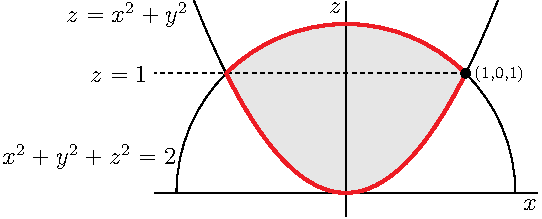
\includegraphics{OE10D_6.pdf}
\end{center}

Let's use cylindrical coordinates to do the two integrals.
In cylindrical coordinates 
\begin{itemize}
\item
$E = \Set{(r\cos\theta,r\sin\theta,z)}{ 0\le r\le 1,\ 0\le\theta\le 2\pi,\ 
                                     r^2\le z\le \sqrt{2-r^2}}$, and
\item
$\dee{V}$ is $r\,\dee{r}\,\dee{\theta}\,\dee{z}$
\end{itemize}
so, for $n=0,1$ (we'll try to do both integrals at the same time)
\begin{align*}
\tripInt_E z^n\ \dee{V}
&=\int_0^1\dee{r} \int_0^{2\pi}\dee{\theta}
   \int_{r^2}^{\sqrt{2-r^2}} \dee{z}\ r\ z^n \\
&=2\pi\int_0^1\dee{r}  \ r\begin{cases}
                  \sqrt{2-r^2}-r^2 & \text{if }n=0 \\
                  \frac{1}{2}\big(2-r^2-r^4\big) & \text{if }n=1
                  \end{cases}
\end{align*}
Since
\begin{align*}
\int_0^1 \dee{r}\ r\sqrt{2-r^2}
&=\left[-\frac{1}{3}(2-r^2)^{3/2}\right]_0^1
=\frac{1}{3}\big(2\sqrt{2}-1\big)
\end{align*}
we have
\begin{align*}
\tripInt_E z^n\ \dee{V}
=2\pi\left.\begin{cases}
\frac{1}{3}(2\sqrt{2}-1)-\frac{1}{4} &\text{if }n=0 \\
\frac{1}{2}-\frac{1}{8}-\frac{1}{12} &\text{if }n=1 
\end{cases}\right\}
=2\pi\begin{cases}
\frac{2}{3}\sqrt{2}-\frac{7}{12} &\text{if }n=0 \\
\frac{7}{24} &\text{if }n=1 
\end{cases}
\end{align*}
and $\bar x=\bar y=0$ and
\begin{align*}
\bar z =\frac{\tripInt_E z\ \dee{V}}{\tripInt_E\dee{V}}
  =\frac{\frac{7}{24}}{\frac{2}{3}\sqrt{2}-\frac{7}{12}}
  =\frac{7}{16\sqrt{2}-14}
  \approx 0.811
\end{align*}
\end{solution}

%%%%%%%%%%%%%%%%%%%%%%%%%%%%%%%%
\begin{question}[M200 2012A] %9
Let $E$ be the smaller of the two solid regions bounded by the surfaces 
$z = x^2 + y^2$ and $x^2 + y^2 + z^2 = 6$. Evaluate
$\tripInt_E (x^2+y^2)\ \dee{V}$ .
\end{question}

%\begin{hint}
%
%\end{hint}

\begin{answer}
$\pi\left[\frac{48}{5}\sqrt{6}-\frac{328}{15}\right] 
\approx 1.65\pi$
\end{answer}

\begin{solution}
Note that both surfaces are invariant under rotations about the
$z$--axis. Here is a sketch of the $y=0$ cross section of E.
\begin{center}
     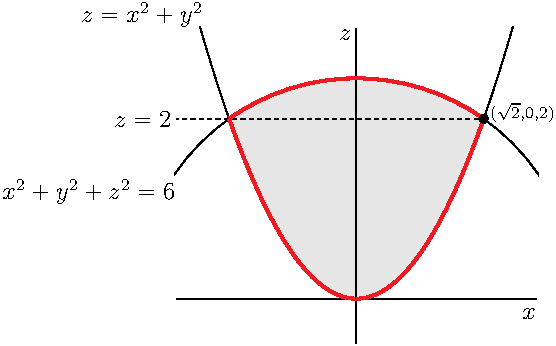
\includegraphics{OE12A_9.pdf}
\end{center}
The surfaces $z = x^2 + y^2$ and $x^2 + y^2 + z^2 = 6$
intersect when $z=x^2+y^2$ and
\begin{equation*}
z+z^2=6
\iff z^2+z-6=0
\iff(z+3)(z-2)=0
\end{equation*}
Since $z=x^2+y^2\ge 0$, the surfaces intersect on the circle $z=2$,
$x^2+y^2=2$. So 
\begin{equation*}
E = \Set{(x,y,z)}{ x^2+y^2\le 2,\ x^2+y^2\le z\le \sqrt{6-x^2-y^2}}
\end{equation*}
Let's use cylindrical coordinates to do the integral.
In cylindrical coordinates 
\begin{itemize}
\item
$E = \Set{(r\cos\theta,r\sin\theta,z)}{ r\le \sqrt{2},\ 0\le\theta\le 2\pi,\ 
                                     r^2\le z\le \sqrt{6-r^2}}$, and
\item
$\dee{V}$ is $r\,\dee{r}\,\dee{\theta}\,\dee{z}$
\end{itemize}
so
\begin{align*}
\tripInt_E (x^2+y^2)\ \dee{V}
&=\int_0^{\sqrt{2}}\dee{r} \int_0^{2\pi}\dee{\theta}
   \int_{r^2}^{\sqrt{6-r^2}} \dee{z}\ r\ r^2 \\
&=2\pi\int_0^{\sqrt{2}}\dee{r}  \ r^3\big(\sqrt{6-r^2}-r^2\big)
 =2\pi\int_0^{\sqrt{2}}\dee{r}\,r\ r^2\sqrt{6-r^2}
   - 2\pi\int_0^{\sqrt{2}}\dee{r}  \ r^5\\
&=2\pi\int_6^4\frac{\dee{u}}{-2}  \ (6-u)\sqrt{u} -2\pi\frac{2^3}{6}
\qquad\text{with } u = 6-r^2,\ \dee{u} = -2r\,\dee{r} \\
&=-\pi\left[6\frac{u^{3/2}}{3/2}-\frac{u^{5/2}}{5/2}\right]_6^4-\frac{8\pi}{3}\\
&=-\pi\left[4\big(8-6\sqrt{6}\big)-\frac{2}{5}\big(32-36\sqrt{6}\big)\right]
             -\frac{8\pi}{3}\\
&=\pi\left[\frac{64}{5}-32-\frac{8}{3} 
         +\left(24-\frac{72}{5}\right)\sqrt{6}\right] \\
&=\pi\left[\frac{48}{5}\sqrt{6}-\frac{328}{15}\right] 
\approx 1.65\pi
\end{align*}
\end{solution}

\begin{question}[M200 2013D] %5
Let $a > 0$ be a fixed positive real number. Consider the solid inside 
both the cylinder $x^2 + y^2 = ax$ and the sphere $x^2 + y^2 + z^2 = a^2$.
Compute its volume.

You may use that 
    $\int \sin^3(\theta) =\frac{1}{12}\cos(3\theta) -\frac{3}{4}\cos(\theta) +C$

\end{question}

%\begin{hint}
%
%\end{hint}

\begin{answer}
$\frac{4a^3}{3}\left[\frac{\pi}{2}  - \frac{2}{3} \right]$
\end{answer}

\begin{solution}
We'll use cylindrical coordinates. In cylindrical coordinates 
\begin{itemize}
\item 
the sphere $x^2+y^2+z^2=a^2$ becomes $r^2+z^2=a^2$ and 
\item 
the circular cylinder  $x^2+y^2=ax$ (or equivalently $(x-a/2)^2+ y^2=a^2/4$)
becomes $r^2=ar\cos\theta$ or $r=a\cos\theta$.
\end{itemize}
Here is a sketch of the top view of the solid.

\begin{center}
     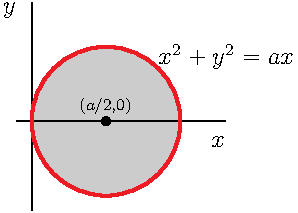
\includegraphics{OE13D_7.pdf}
\end{center}

The solid is
\begin{equation*}
\Set{(r\cos\theta\,,\,r\sin\theta\,,\,z)}{
        -\nicefrac{\pi}{2}\le\theta\le\nicefrac{\pi}{2}\,,\,
        0\le r\le a\cos\theta\,,\,
        -\sqrt{a^2-r^2}\le z\le \sqrt{a^2-r^2}}
\end{equation*}
By symmetry, the volume of the specified solid is four times
the volume of the solid
\begin{equation*}
\Set{(r\cos\theta\,,\,r\sin\theta\,,\,z)}{
        0\le\theta\le\nicefrac{\pi}{2}\,,\,
        0\le r\le a\cos\theta\,,\,
        0\le z\le \sqrt{a^2-r^2}}
\end{equation*}
Since $\dee{V} = r\,\dee{r}\,\dee{\theta}\,\dee{z}$,
 the volume of the solid is
\begin{align*}
4\int_0^{\pi/2}\dee{\theta} \int_0^{a\cos\theta} \dee{r}
   \int_0^{\sqrt{a^2-r^2}}\dee{z}\ r
&=4\int_0^{\pi/2}\dee{\theta} \int_0^{a\cos\theta} \dee{r}\ 
        r\sqrt{a^2-r^2} \\
&=-\frac{4}{3}\int_0^{\pi/2}\dee{\theta}\ 
         \big(a^2-r^2\big)^{3/2}\Big|_0^{a\cos\theta} \\
&=\frac{4}{3}\int_0^{\pi/2}\dee{\theta}\ 
         \Big[a^3-\big(a^2-a^2\cos^2\theta\big)^{3/2}\Big] \\
&=\frac{4a^3}{3}\int_0^{\pi/2}\dee{\theta}\ 
         \big[1-\sin^3\theta\big] \\
&=\frac{4a^3}{3}\left[\theta - \frac{1}{12}\cos(3\theta) + \frac{3}{4}\cos\theta
           \right]_0^{\pi/2} \\
&=\frac{4a^3}{3}\left[\frac{\pi}{2} + \frac{1}{12} - \frac{3}{4} \right] \\
&=\frac{4a^3}{3}\left[\frac{\pi}{2}  - \frac{2}{3} \right]
\end{align*}
\end{solution}

\begin{question}[M200 2014A] %7
Let $E$ be the solid lying above the surface $z = y^2$ and below 
the surface $z = 4 - x^2$. Evaluate
\begin{equation*}
\tripInt_E y^2\ \dee{V}
\end{equation*}
You may use the half angle formulas:
\begin{equation*}
\sin^2\theta = \frac{1-\cos(2\theta)}{2},\qquad
\cos^2\theta = \frac{1+\cos(2\theta)}{2}
\end{equation*}
\end{question}

%\begin{hint}
%
%\end{hint}

\begin{answer}
$\frac{16\pi}{3}$
\end{answer}

\begin{solution}
Note that the surfaces meet when $z=y^2=4-x^2$ and then $(x,y)$
runs over the circle $x^2+y^2=4$. So the domain of integration is
\begin{equation*}
E = \Set{(x,y,z)}{x^2+y^2\le 4,\ y^2\le z\le 4-x^2}
\end{equation*}
Let's switch to cylindrical coordinates. Then
\begin{equation*}
E = \Set{(r\cos\theta,r\sin\theta,z)}{0\le r\le 2,\ 0\le\theta\le 2\pi,
            \ r^2\sin^2\theta\le z\le 4-r^2\cos^2\theta}
\end{equation*}
and, since $\dee{V} = r\,\dee{r}\,\dee{\theta}\,\dee{z}$,
\begin{align*}
\tripInt_E y^2\ \dee{V}
&=\int_0^2\dee{r} \int_0^{2\pi} \dee{\theta}
         \int_{r^2\sin^2\theta}^{4-r^2\cos^2\theta}\dee{z}\ r\ 
         \overbrace{r^2\sin^2\theta}^{y^2} \\
&=\int_0^2\dee{r} \int_0^{2\pi} \dee{\theta}\ 
             r^3\sin^2\theta\big[4-r^2\cos^2\theta - r^2\sin^2\theta\big]
   \displaybreak[0]\\
&=\int_0^2\dee{r}\ \big[4r^3-r^5\big] \int_0^{2\pi} \dee{\theta}\ 
         \frac{1-\cos(2\theta)}{2}  \displaybreak[0]\\
&=\frac{1}{2}\int_0^2\dee{r}\ \big[4r^3-r^5\big]\ 
      \left[\theta-\frac{\sin(2\theta)}{2}\right]_0^{2\pi}  \displaybreak[0]\\
&=\pi\left[r^4-\frac{r^6}{6}\right]_0^2 \\
&=\frac{16\pi}{3}
\end{align*}
For an efficient, sneaky, way to evaluate 
$\int_0^{2\pi}\sin^2\theta\ \dee{\theta}$,
see Remark \eref{CLP200}{rem sneaky} in the CLP-3 text.
\end{solution}

%%%%%%%%%%%%%%%%%%%%%%%%%%%%%%%%%%%%%%%%%
\begin{question}
The centre of mass $(\bar x,\bar y, \bar z)$ of a body $B$ having
density $\rho(x,y,z)$ (units of mass per unit volume) at $(x,y,z)$ is defined
to be
\begin{equation*}
\bar x=\frac{1}{M}\tripInt_B x\rho(x,y,z)\ \dee{V}\quad
\bar y=\frac{1}{M}\tripInt_B y\rho(x,y,z)\ \dee{V}\quad
\bar z=\frac{1}{M}\tripInt_B z\rho(x,y,z)\ \dee{V}
\end{equation*}
where
\begin{equation*}
M=\tripInt_B \rho(x,y,z)\ \dee{V}
\end{equation*}
is the mass of the body. So, for example, $\bar x$ is the weighted average
of $x$ over the body. Find the centre of mass of the part of the solid
ball $x^2+y^2+z^2\le a^2$ with $x\ge 0$, $y\ge 0$ and $z\ge 0$, assuming
that the density $\rho$ is constant.
\end{question}

\begin{hint}
Use cylindrical coordinates.
\end{hint}

\begin{answer}
$\bar x=\bar y=\bar z=\frac{3}{8}a$
\end{answer}

\begin{solution}
By symmetry, $\bar x=\bar y=\bar z$, so it suffices to compute,
for example, $\bar z$.   The mass of the body is the density, $\rho$,
times its volume, which is one eighth of the volume of a sphere. So
\begin{equation*}
M=\frac{\rho}{8}\ \frac{4}{3}\pi a^3
\end{equation*}
In cylindrical coordinates, the equation of the spherical surface of the
body is $r^2+z^2=a^2$. The part of the body at height $z$ above the 
$xy$--plane is one quarter of a disk of radius $\sqrt{a^2-z^2}$. The numerator
of $\bar z$ is
\begin{alignat*}{3}
\tripInt_B z\rho\ \dee{V}
&=\rho\int_0^a \dee{z}\int_0^{\pi/2}d\theta\int_0^{\sqrt{a^2-z^2}}dr\ r\ z
&&=\rho\int_0^a \dee{z}\int_0^{\pi/2}d\theta\ z\ \frac{r^2}{2}
                                   \bigg|_0^{\sqrt{a^2-z^2}} \\
&=\frac{\rho}{2}\int_0^a \dee{z}\int_0^{\pi/2}d\theta\ z(a^2-z^2)
&&=\frac{\pi}{4}\rho\int_0^a \dee{z}\ z(a^2-z^2) \\
&=\frac{\pi}{4}\rho\left[a^2\frac{z^2}{2}-\frac{z^4}{4}\right]_0^a 
=\frac{\pi}{16}\rho a^4
\end{alignat*}
Dividing by $M=\frac{\pi}{6}\rho a^3$ gives 
$\bar x=\bar y=\bar z=\frac{3}{8}a$.
\end{solution}

%%%%%%%%%%%%%%%%%%%%%%%%%%%%%%%%
\begin{question}[M200 2003D] %7
A sphere of radius $2{\rm m}$ centred on the origin has variable density 
$\frac{5}{\sqrt{3}}(z^2+1)$kg/${\rm m}^3$. A hole of diameter 1m is drilled
through the sphere along the $z$--axis.
\begin{enumerate}[(a)]
\item
Set up a triple integral in cylindrical coordinates giving
the mass of the sphere after the hole has been drilled.
\item
 Evaluate this integral.
\end{enumerate}
\end{question}

%\begin{hint}
%\end{hint}

\begin{answer}
(a) $\dst\text{mass} = 
\int_{1/2}^2 \dee{r} \int_{-\sqrt{4-r^2}}^{\sqrt{4-r^2}} \dee{z}\int_0^{2\pi}\dee{\theta}\ 
\frac{5}{\sqrt{3}}(z^2+1)r$

(b) $\frac{525}{24}\sqrt{5}\pi\approx 153.7\text{kg}$
\end{answer}

\begin{solution}
(a) In cylindrical coordinates the equation of a sphere of radius
2 centred on the origin is $r^2+z^2=2^2$. Since 
$\dee{V}=r\, \dee{r}\, \dee{\theta}\, \dee{z}$
and $\dee{m} =\frac{5}{\sqrt{3}}(z^2+1)r\, \dee{r}\, \dee{\theta}\, \dee{z}$ 
and the hole has radius $1/2$, the integral is
\begin{align*}
\text{mass} = 
\int_{1/2}^2 \dee{r} \int_{-\sqrt{4-r^2}}^{\sqrt{4-r^2}} \dee{z}\int_0^{2\pi}\dee{\theta}\ 
\frac{5}{\sqrt{3}}(z^2+1)r
\end{align*}

(b)
By part (a)
\begin{align*}
\text{mass} = 
\int_{1/2}^2 \dee{r} \int_{-\sqrt{4-r^2}}^{\sqrt{4-r^2}} \dee{z}\int_0^{2\pi}\dee{\theta}\ 
\frac{5}{\sqrt{3}}(z^2+1)r
&=4\pi\frac{5}{\sqrt{3}}\int_{1/2}^2\dee{r}\ r\int_0^{\sqrt{4-r^2}}\dee{z}\ (z^2+1) \\
&=4\pi\frac{5}{\sqrt{3}}\int_{1/2}^2\dee{r}\ 
                   r\left[\frac{z^3}{3}+z\right]_0^{\sqrt{4-r^2}} \\
&=4\pi\frac{5}{\sqrt{3}}\int_{1/2}^2\dee{r}\ 
           r\left[\frac{1}{3}{(4-r^2)}^{3/2}+{(4-r^2)}^{1/2}\right] 
\end{align*}
Make the change of variables $s=4-r^2$, $\dee{s}=-2r\,\dee{r}$. This gives
\begin{align*}
\text{mass} &= 4\pi\frac{5}{\sqrt{3}}\int_{15/4}^0\frac{\dee{s}}{-2}\   
                         \left[\frac{1}{3}s^{3/2}+s^{1/2}\right]
= -2\pi\frac{5}{\sqrt{3}} 
\left[\frac{2}{15}s^{5/2}+\frac{2}{3}s^{3/2} \right]_{15/4}^0 \\
&=
2\pi\frac{5}{\sqrt{3}} \left[\frac{2}{15}\frac{15^{5/2}}{32}
+\frac{2}{3}\frac{15^{3/2}}{8}\right] \\
&=2\pi\frac{5}{\sqrt{3}} \left[\frac{1}{16}+\frac{1}{12}\right]15^{3/2}
=\frac{525}{24}\sqrt{5}\pi\approx 153.7\text{kg}
\end{align*}
\end{solution}

%%%%%%%%%%%%%%%%%%%%%%%%%%%%%%%%%%%%%%%%%
\begin{question} [M200 2001A] % 7
Consider the finite solid bounded by the three surfaces:
$z=e^{-x^2-y^2}$, $z=0$ and $x^2+y^2=4$.
\begin{enumerate}[(a)]
\item 
Set up (but do not evaluate) a triple integral in rectangular
coordinates that describes the volume of the solid.

\item
Calculate the volume of the solid using any method.
\end{enumerate}
\end{question}

%\begin{hint}
%
%\end{hint}

\begin{answer}
(a) $\dst\int_{-2}^2 \dee{x}
    \int_{-\sqrt{4-x^2}}^{\sqrt{4-x^2}}\dee{y}\int_0^{e^{-x^2-y^2}}\dee{z}$
\qquad
(b) $\pi\big[1-e^{-4}\big]\approx 3.084$
\end{answer}

\begin{solution}
(a) The solid consists of all $(x,y,z)$ with
\begin{itemize}
\item
$(x,y)$ running over the disk $x^2+y^2\le 4$ and
\item
for each fixed $(x,y)$ obeying $x^2+y^2\le 4$, $z$ running from
$0$ to $e^{-x^2-y^2}$
\end{itemize}
On the disk $x^2+y^2\le 4$,
\begin{itemize}
\item
$x$ runs from $-2$ to $2$ and
\item
for each fixed $x$ obeying $-2\le x\le 2$, $y$ runs from
$-\sqrt{4-x^2}$ to $\sqrt{4-x^2}$
\end{itemize}
So
\begin{equation*}
\text{Volume}=\int_{-2}^2 \dee{x}
    \int_{-\sqrt{4-x^2}}^{\sqrt{4-x^2}}\dee{y}\int_0^{e^{-x^2-y^2}}\dee{z}
\end{equation*}

(b) Switching to cylindrical coordinates
\begin{align*}
\text{Volume}&=\int_0^2 \dee{r}\int_0^{2\pi}\dee{\theta} \int_0^{e^{-r^2}}\dee{z}\ r
=\int_0^2 \dee{r}\int_0^{2\pi}\dee{\theta} \ r e^{-r^2}
=\int_0^2 \dee{r}\ 2\pi\ r e^{-r^2} \\
&=-\pi e^{-r^2}\Big|_0^2
=\pi\big[1-e^{-4}\big]\approx 3.084
\end{align*}
\end{solution}

%%%%%%%%%%%%%%%%%%%%%%%%%%%%%%%%%%%%%%%%%
\begin{question} [M200 2000A] % 9
Find the volume of the solid which is inside $x^2 + y^2 = 4$,
above $z = 0$ and below $2z = y$.
\end{question}

%\begin{hint}
%
%\end{hint}

\begin{answer}
$\frac{8}{3}$
\end{answer}

\begin{solution}
The solid consists of the set of all points $(x,y,z)$ such
that $x^2+y^2\le 4$ and $0\le z\le\frac{y}{2}$. In particular $y\ge 0$.
When we look at the solid from above, we see all $(x,y)$ with
$x^2+y^2\le 4$ and $y\ge 0$. This is sketched in the figure on the left
below.
\begin{center}
     \raisebox{0.5\height}{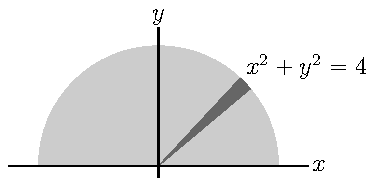
\includegraphics{OE00AQ9a.pdf}}\qquad
     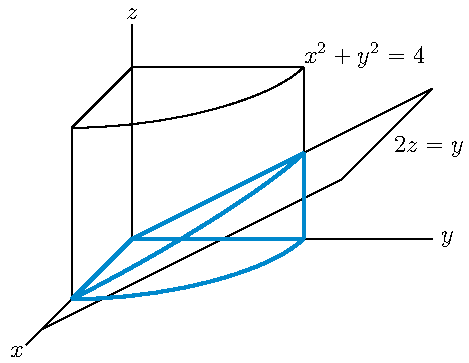
\includegraphics{OE00AQ9b.pdf}
\end{center}   
We'll use cylindrical coordinates. In the base region (the shaded region
in the figure on the left above)
\begin{itemize}
\item
$\theta$ runs from $0$ to $\pi$ and
\item
for each fixed $\theta$ between $0$ and $\pi$, $r$ runs from $0$ to $2$.
\item
For each fixed point $(x,y)=(r\cos\theta,r\sin\theta)$ in the base
region, $z$ runs from $0$) to $\frac{y}{2}=\frac{r\sin\theta}{2}$.
\end{itemize}
So the volume is
\begin{align*}
\int_0^\pi \dee{\theta}\int_0^2 \dee{r}\int_0^{r\sin\theta/2} dz\ r
&=\int_0^\pi \dee{\theta}\int_0^2 \dee{r}\ \frac{1}{2} r^2\sin\theta
=\int_0^\pi \dee{\theta}\ \frac{r^3}{6}\sin\theta\,\bigg|_0^2
=\frac{4}{3}\int_0^\pi \dee{\theta}\ \sin\theta \\
&=-\frac{4}{3}\cos\theta\,\bigg|_0^\pi
=\frac{8}{3}
\end{align*}
\end{solution}





%%%%%%%%%%%%%%%%%%
\subsection*{\Application}
%%%%%%%%%%%%%%%%%%

\begin{question}[M200 2014D] %7
The density of hydrogen gas in a region of space is given by the formula
\begin{equation*}
\rho(x,y,z) =\frac{z+2x^2}{1+x^2+y^2}
\end{equation*}
\begin{enumerate}[(a)]
\item
At $(1,0,-1)$, in which direction is the density of hydrogen increasing 
most rapidly?
\item
You are in a spacecraft at the origin. Suppose the spacecraft flies 
in the direction of $\llt 0,0,1\rgt$. It has a disc of radius $1$, 
centred on the spacecraft and deployed perpendicular to the direction 
of travel, to catch hydrogen. How much hydrogen has been collected
by the time that the spacecraft has traveled a distance $2$? 

You may use the fact that $\int_0^{2\pi}\cos^2\theta\ \dee{\theta}
=\pi$.
\end{enumerate}
\end{question}

%\begin{hint}
%
%\end{hint}

\begin{answer}
(a) The unit vector in the direction of maximum rate of increse is $\frac{1}{\sqrt{10}}(3,0,1)$.

(b) $2\pi$
\end{answer}

\begin{solution}
(a) The direction of maximum rate of increase is $\vnabla\rho(1,0,-1)$.
As
\begin{align*}
\pdiff{\rho}{x}(x,y,z)
      &= \frac{4x}{1+x^2+y^2} -\frac{2x(z+2x^2)}{{(1+x^2+y^2)}^2} &
\pdiff{\rho}{x}(1,0,-1)
      &= \frac{4}{2} -\frac{2(-1+2)}{{(2)}^2} =\frac{3}{2}
\\
\pdiff{\rho}{y}(x,y,z)
      &=  -\frac{2y(z+2x^2)}{{(1+x^2+y^2)}^2} &
\pdiff{\rho}{y}(1,0,-1)
      &=  0\\
\pdiff{\rho}{z}(x,y,z)
      &= \frac{1}{1+x^2+y^2} &
\pdiff{\rho}{z}(1,0,-1)
      &= \frac{1}{2}  
\end{align*}
So $\vnabla\rho(1,0,-1) = \frac{1}{2}(3,0,1)$. The unit vector
in this direction is $\frac{1}{\sqrt{10}}(3,0,1)$.

(b) The region swept by the space craft is, in cylindrical coordinates,
\begin{equation*}
   V=\Set{(r\cos\theta\,,\,r\sin\theta\,,\,z)}{0\le\theta\le 2\pi,\ 
             0\le r\le 1,\ 
              0\le z\le 2}
\end{equation*}
and the amount of hydrogen collected is
\begin{align*}
\tripInt_V \rho\ \dee{V} &=\tripInt_V\frac{z+2r^2\cos^2\theta}{1+r^2}r\dee{r}\,\dee{\theta}\,\dee{z} \\
&=\int_0^2\dee{z} \int_0^{2\pi} \dee{\theta} \int_0^1\dee{r}\ 
              \frac{zr+(2\cos^2\theta)r^3}{1+r^2} \\
&=\int_0^2\dee{z} \int_0^{2\pi} \dee{\theta} \int_0^1\dee{r}\ 
     \left[ z \frac{r}{1+r^2} +2r\cos^2\theta 
               -\cos^2\theta\frac{2r}{1+r^2}\right]\\
&\hskip1.5in\text{since }\frac{r^3}{1+r^2} = \frac{r+r^3 - r}{1+r^2}
                         =r-\frac{r}{1+r^2} \\
&=\int_0^2\dee{z} \int_0^{2\pi} \dee{\theta}\ 
              \left[\frac{z}{2}\ln(1+r^2)+r^2\cos^2\theta
                     -\ln(1+r^2)\cos^2\theta\right]_0^1 \\
&=\int_0^2\dee{z} \int_0^{2\pi} \dee{\theta}\ 
              \left[\frac{\ln 2}{2} z+ \cos^2\theta
                     -\ln(2)\cos^2\theta\right] \\
&=\int_0^2\dee{z} \ \left[(\pi\ln 2) z+ \pi-\pi\ln 2\right] \\
&= 2\pi\ln 2 +2\pi -2\pi\ln 2 \\
&=2\pi
\end{align*}
\end{solution}

%%%%%%%%%%%%%%%%%%%%%%%%%%%%%%%%%%%%%%%%%
\begin{question}
A torus of mass $M$ is generated by rotating a circle of radius $a$ about an axis in its plane at distance $b$ from the centre $(b>a)$. The
torus has constant density.
Find the moment of inertia about the axis of rotation.
By definition the moment of intertia is $\tripInt r^2 \dee{m}$ 
where $\dee{m}$ is the mass of an infinitesmal piece of the solid and $r$ is 
its distance from the axis.
\end{question}

%\begin{hint}
%
%\end{hint}

\begin{answer}
$M\big(\frac{3}{4}a^2+b^2\big)$
\end{answer}

\begin{solution}
 We may choose our coordinate axes so that the torus is constructed by rotating the circle $(x-b)^2+z^2=a^2$
(viewed as lying in the $xz$--plane) about the $z$--axis. On this circle,
$x$ runs from $b-a$ to $b+a$. 
\vadjust{
\begin{center}
     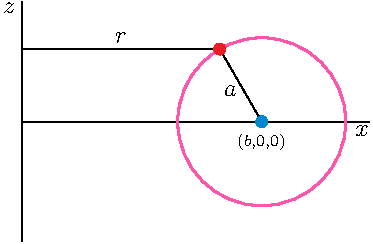
\includegraphics{torusSection.pdf}
\end{center}
}%
In cylindrical coordinates, the torus has equation $(r-b)^2+z^2=a^2$. 
(Recall that the cylindrical coordinate $r$ of a point is its distance from the 
$z$--axis.)
On this torus, 
\begin{itemize}
\item $r$ runs from $b-a$ to $b+a$. 
\item For each fixed $r$, $z$ runs
from $-\sqrt{a^2-(r-b)^2}$ to $\sqrt{a^2-(r-b)^2}$. 
\end{itemize}
As the torus
is symmetric about the $xy$--plane, its volume is twice that of the volume 
of the part with $z\ge 0$. 
\begin{align*}
\text{Volume}
&= 2\int_{0}^{2\pi} d\theta\int_{b-a}^{b+a}\dee{r}\ r\int_{0}^{\sqrt{a^2-(r-b)^2}}\dee{z} \\
&= 2\int_{0}^{2\pi} d\theta\int_{b-a}^{b+a}\dee{r}\ r\sqrt{a^2-(r-b)^2} \\
&= 4\pi \int_{-a}^{a}\dee{s}\ (s+b)\sqrt{a^2-s^2}
\qquad\text{ where $s=r-b$}
\end{align*}
As $s\sqrt{a^2-s^2}$ is odd under $s\rightarrow -s$, 
$\int_{-a}^{a}\dee{s}\ s\sqrt{a^2-s^2}=0$. Also,  $\int_{-a}^{a}\dee{s}\ \sqrt{a^2-s^2}$
is precisely the area of the top half of a circle of radius $a$. So
$$
\text{Volume }= 4b\pi \int_{-a}^{a}\dee{s}\ \sqrt{a^2-s^2}
=2\pi^2a^2b
$$
So the mass density of the torus is $\frac{M}{2\pi^2a^2b}$ and
$\dee{m} = \frac{M}{2\pi^2a^2b}\,\dee{V}
          =\frac{M}{2\pi^2a^2b}\,r\,\dee{r}\,d\theta\,\dee{z}$ 
and
\begin{align*}
\text{moment of inertia}
&= 2\int_{0}^{2\pi} d\theta\int_{b-a}^{b+a}\dee{r}\ r\int_{0}^{\sqrt{a^2-(r-b)^2}}\dee{z}\ 
\frac{M}{2\pi^2a^2b} r^2 \\
&= \frac{M}{\pi^2a^2b}\int_{0}^{2\pi} d\theta\int_{b-a}^{b+a}\dee{r}\ r^3\sqrt{a^2-(r-b)^2} \\
&= \frac{2M}{\pi a^2b} \int_{-a}^{a}\dee{s}\ (s+b)^3\sqrt{a^2-s^2}
\qquad\text{ where $s=r-b$} \\
&= \frac{2M}{\pi a^2b} \int_{-a}^{a}\dee{s}\ (s^3+3s^2b+3sb+b^3)\sqrt{a^2-s^2}
\end{align*}
Again, by oddness, the $s^3$ and $3sb$ integrals are zero. For the others,
substitute in $s=a\sin t$, $\dee{s}=a\cos t$.
\begin{align*}
\text{moment}
&= \frac{2M}{\pi a^2b} \int_{-{\pi\over 2}}^{{\pi\over 2}}(a\cos t\, \dee{t}) 
\ (3a^2b\sin^2 t+b^3)a\cos t
= \frac{2M}{\pi } \int_{-{\pi\over 2}}^{{\pi\over 2}}\dee{t}\  
(3a^2\sin^2 t+b^2)\cos^2 t \\
&= \frac{4M}{\pi} \int_0^{{\pi\over 2}}\dee{t}\ 
(3a^2\cos^2 t-3a^2\cos^4 t+b^2\cos^2 t)
      \qquad\text{since $\sin^2t=1-\cos^2t$} 
\end{align*}
To integrate\footnote{For a general discussion of trigonometric integrals see
\S\eref{CLP101}{sec trigint} in the CLP-2 text. In particular the integral  
$\int \cos^4 x\ \dee{x}$ is evaluated in Example \eref{CLP101}{eg:TRGINTc} 
in the CLP-2 text. For an efficient, sneaky, way to evaluate 
$\int_0^{{\pi\over 2}} \cos^2 t\ \dee{t}$
see Remark \eref{CLP200}{rem sneaky} in the CLP-3 text.} 
$\cos^2t$ and $\cos^4t$, we use the double angle formulae
$\sin^2 x= \frac{1-\cos(2x)}{2}$ and $\cos^2 x= \frac{1+\cos(2x)}{2}$
to write
\begin{equation*}
\cos^2 t= \frac{1+\cos(2t)}{2}
\end{equation*}
and 
\begin{align*}
  \cos^4 t &= \left[ \frac{1+\cos(2t)}{2} \right]^2 \\
   &= \frac{1}{4} + \frac{1}{2} \cos(2t) + \frac{1}{4}\cos^2(2t)\\
  &= \frac{1}{4} + \frac{1}{2} \cos(2t) + \frac{1}{8}\left(1 + \cos(4t)\right)\\
  &= \frac{3}{8} + \frac{1}{2} \cos(2t) + \frac{1}{8}\cos(4t)
\end{align*}
So
\begin{align*}
\text{moment}
&= \frac{4M}{\pi} 
\left[3a^2\left(\frac{t}{2}+\frac{\sin(2t)}{4}\right)
    -3a^2\left(\frac{3t}{8} + \frac{1}{4} \sin(2t) + \frac{1}{32}\sin(4t)\right)
    +b^2\left(\frac{t}{2}+\frac{\sin(2t)}{4}\right)\right]_0^{{\pi\over 2}} \\
&= \frac{4M}{\pi} 
         \Big[3a^2\frac{\pi}{4}-3a^2\frac{3\pi}{16}+b^2\frac{\pi}{4}\Big]
=M\left(\frac{3}{4}a^2+b^2\right)
\end{align*}

\end{solution}
